
\item A thin ring of mass \(2 \, \text{kg}\) and radius \(0.5 \, \text{m}\) is rolling without slipping on a horizontal plane with velocity \(1 \, \text{m/s}\). A small ball of mass \(0.1 \, \text{kg}\), moving with velocity \(20 \, \text{m/s}\) in the opposite direction, hits the ring at a height of \(0.75 \, \text{m}\) and goes vertically up with velocity \(10 \, \text{m/s}\). Immediately after the collision
    \begin{center}
        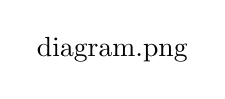
\begin{tikzpicture}
            \node at (0, 0) {diagram.png};
        \end{tikzpicture}
    \end{center}
    \begin{tasks}(2)
        \task the ring has pure rotation about its stationary CM.
        \task the ring comes to a complete stop.
        \task friction between the ring and the ground is to the left.
        \task there is no friction between the ring and the ground.
    \end{tasks}
